\chapter{Introduction} \label{chapter:introduction}

Infineon technologies Austria is one of the leading semiconductor companies worldwide. With around 4,820 employees, the company makes an important contribution to shaping the digital and networked future. Through the development of microelectronics and their constant improvement, Infineon enables efficient energy management, intelligent mobility and secure, seamless communication. \newline

\section{Motivation}
Detection and localization of faults in semiconductors is a knowledge-intensive and tedious task. To increase the chances of success, an electrical engineer should be able to get all available information about the samples of similar past jobs. Various support systems used in Failure Analysis (FA), like databases, wikis, or file shares, often have this information stored as documents describing previous analysis reports of similar samples, best practices, specifications, customer reports, etc. However, accessing knowledge contained in these documents can be problematic, since in most cases, such support systems only provide rudimentary search functionality, like keyword matching. As a result, to find relevant information about jobs similar to the considered one, an engineer must query multiple systems, manually evaluate returned reports looking for similar characteristics, and asserting the value of each document for the current problem. Furthermore, the report corpus includes a quantity of over one million documents, which means a long search time if you are looking for a specific topic. These procedure is depicted in Figure \ref{fig:fa_process}

\begin{figure}[H]
	\centering
	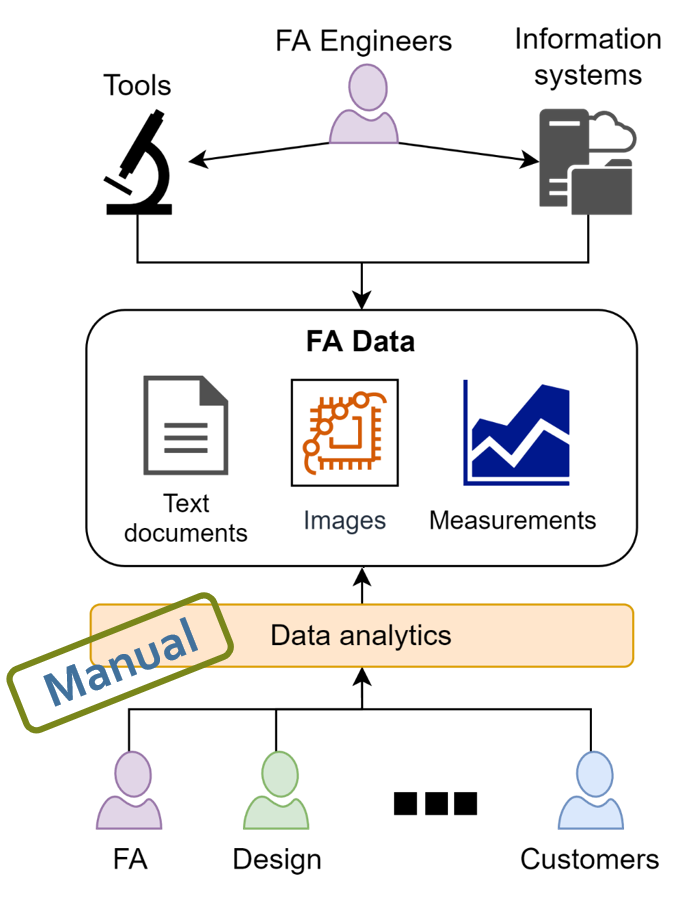
\includegraphics[width=0.3\textwidth]{figures/fa_process.png}
	\caption{FA Analysis Process}
	\label{fig:fa_process}
\end{figure}

In order to accelerate this process of troubleshooting and to make it easier to find similarities between past and new jobs, the integration of artificial intelligence in the failure analysis process is suitable. Integrating AI into Infineons failure analysis could look like in Figure \ref{fig:ai_process} where AI infrastructures are used to load and process ressources and help not only FA employees, but all Infineon employees and customers to better understand the existing data through appropriate processing and to be able to use it in a targeted manner.

\begin{figure}[H]
	\centering
	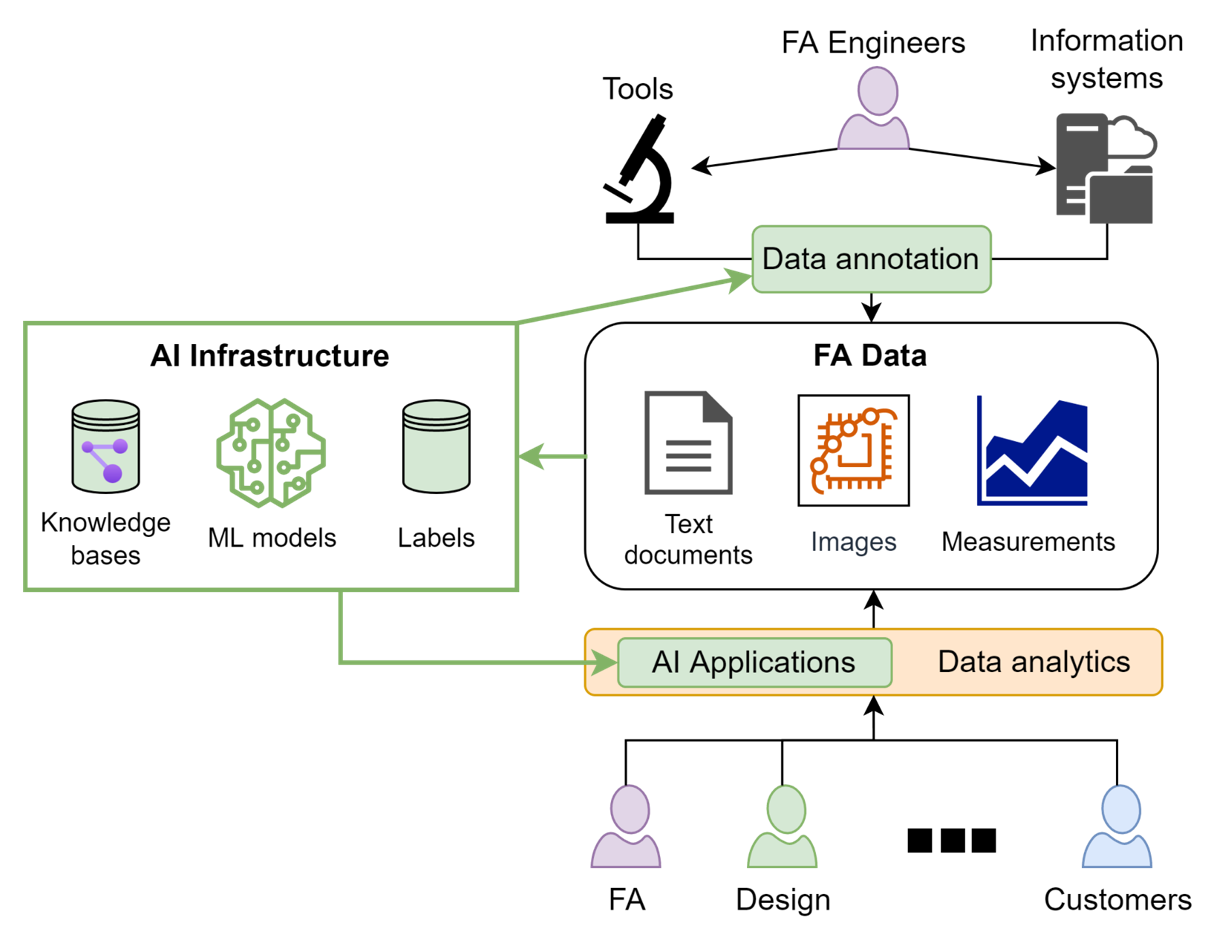
\includegraphics[width=0.6\textwidth]{figures/ai_process_idea.png}
	\caption{FA Analysis Process with AI Integration}
	\label{fig:ai_process}
\end{figure}

Modern Natural Language Processing methods (NLP) already showed their efficiency in various applications, including automatic translators, Recommender Systems or chatbots. Among these applications, text classification is one of the most promising to solve the FA search problem by automatically associating labels with a report denoting physical or electrical faults described in it, applied methods and tools, etc. The engineers can then use these labels to perform various tasks, like identifying similar jobs or getting statistics on possible faults, tools, or methods. \newline
This is why one of the first applications of Artificial Intelligence (AI) tools at the FA laboratory of Infineon consisted on a classifier of the FA reports. To support the classifier and improve performance as best as possible, a language model is trained on in-domain text data as shown in Figure \ref{fig:fa_bert_process}. The model should support engineers during the analysis and report writing process.

\begin{figure}[H]
	\centering	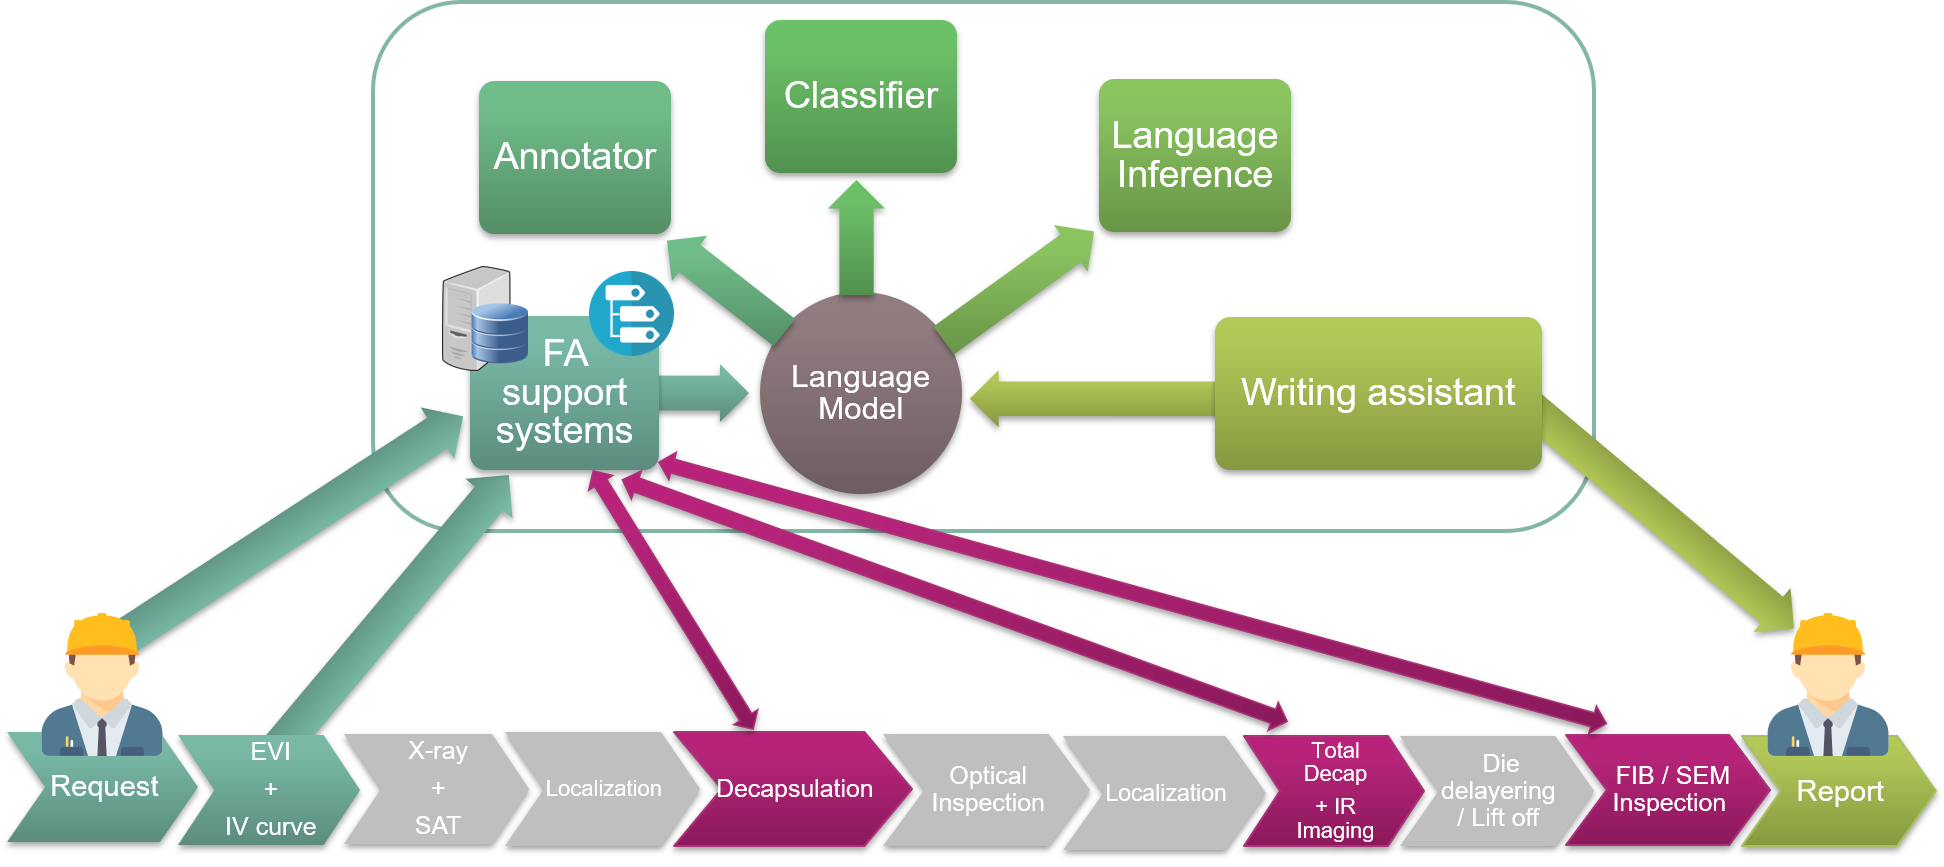
\includegraphics[width=1\textwidth]{figures/fa_bert_process.png}
	\caption{FA-BERT Integration into FA Analysis Prozess}
	\label{fig:fa_bert_process}
\end{figure}



\section{Problem Description}
The goal of this project is to develop a FA report classifier with a BERT model.
In order to do so, the task has been divided into two phases: \newline
First, we have developed a Language Model based on the state-of-the-art model BERT. Therefore we had to consider our specific domain and select the most appropriate model for our domain. Since many successors of BERT have been developed but none of them aimed at the electrical domain, we had to select a model as close as possible to our field of study in order to achieve a satisfying performance later. \newline
Second, we focused on defining the structure of the classifier, which consisted on the BERT network and additional classification layers. To test the results, we have defined a series of classification problems based on the FA reports. \newline
Given the nature of this project the two phases were developed in parallel so the joint performance hasn't been tested yet. \newline

\section{Research Questions}
This thesis will address the following research questions:
\begin{itemize}
	\item What kind of BERT models already exist and which one to choose as an entrypoint for training?
	\item What data should be used for further training and how to collect it?
	\item How to train and evaluate the resulting model?
\end{itemize}

The following chapters in this thesis will cover the research questions described above. Before that, as a basis for the content that follows, some terms and topics related to natural language processing will be discussed.

\section{Contributions}
\textbf{RQ1: What kind of BERT models already exist and which one to choose as an entrypoint for training?} \newline
In order to fulfill the goal of developing an innovative language model trained on the semiconductor domain, it was necessary to find an existing language model which has already been trained on english text similar to electrical engineering or semiconductor topics. With this language model to use as entry point for our training, we assumed it would be easier to achieve our desired goals. 
After extensive search and research, we found possible candidates for the model entry point. One of the largest BERT models is Med-BERT, which has been trained on medical and biomedical documents. Unfortunately, this model is not suitable as a starting point for our training, since words in medical texts are very similar to those in semiconductor texts but have a different semantic meaning. Because of this, the model can become "confused" when trying to understand the text. Other promising models are SciBERT and S2ORC-SciBERT. Both models are trained using scientific, english texts, with the training corpus consisting of chemistry, physics, but also mainly medical topics. In contrast to SciBERT, S2ORC-SciBERT has a slightly larger vocabulary and was also trained on a larger data set, which also includes topics such as computer science and engineering. \newline
After some evaluation processes on error analysis reports, S2ORC-SciBERT could be chosen as the entry point. The performance of S2ORC-SciBERT is slightly better than that of SciBERT.

\textbf{RQ2: What data should be used for further training and how to collect it?} \newline
To further train the language model entrypint on a domain specific dataset to achieve the desired results, the specific dataset had to be collected and transformed into a shape which allows to train a BERT based language model. To collect the domain specific texts, we used \textit{GoogleScholar}, \textit{SemanticScholar} and \textit{IEEE} to download as many papers as possible. Also we used parts of the S2ORC dataset and filtered for texts with the topics chemistry, physics, computer science, mathematical science and engineering. After collecting the papers, the raw text had to be extracted. Therefore we were allowed to use a text extractor tool developed by Infineon collegues in Bangalore and did not had to develop it on our own. The raw text had been saved in csv files and could be loaded to create a okenized dataset ready for training. In total the training data frame included 1 783 789 rows which is about 10GB of data.


\textbf{RQ3: How to train and evaluate the resulting model?} \newline
As a training method we decided to choose the most common way of how to pretrain a BERT-based model: using Masked Language Modeling. This technique had already been used for training the original BERT model and will now also been used in an adapted way for our training experiments. In order to achieve a satisfying result, we wanted our model to understand the FA reports as good as possible. With the whole-word-masking technique, which is an adaption of the traditional masked language modeling algorithm, we achieved a lower loss during training. The evaluation of the final model on the FA report job summaries show, that our trained model has a better understanding of the texts than the initial model.